\documentclass[dvipsnames]{beamer}
\usepackage[T1]{fontenc}
\usepackage{geometry}
\usepackage[utf8]{inputenc}
\usepackage{colortbl}
\usepackage[english]{babel}
\usepackage{pgf}
%\usepackage{beamerthemesplit}
\usepackage{graphicx,epsfig, subfigure}
\usepackage{hyperref}
%\usepackage{srcltx}
\usepackage{multirow}
\usepackage{minted}
\definecolor{lightgray}{rgb}{.3,.3,.3}

\usepackage{niceslides}

\title{A Dependently Timed Drum Machine Language}
\author{Joachim Tilsted Kristensen\\ \texttt{joachim.tilsted@gmail.com}}
\institute{Functional Programming Talks\\ Chalmers University of Technology}

\date{22/08-2021}

%\setlength{\parskip}{\baselineskip}

\def\Var{\ensuremath{\text{\bf Var}}}
\def\Con{\ensuremath{\text{\bf Con}}}
\def\N{\ensuremath{\mathbb N}}
\def\R{\ensuremath{\mathbb R}}
\def\Q{\ensuremath{\mathbb Q}}
\def\OR{\ensuremath{\ |\ }}
\def\TO{\ensuremath{\rightarrow}}
\def\LB{\ensuremath{\llbracket}}
\def\RB{\ensuremath{\rrbracket}}
\newcommand\LIT[1]{\ensuremath{\text{\tt #1}}}
\newcommand\SLIT[1]{\ \LIT{#1}\ }
\newcommand\IF[3]{\LIT{if}\ #1\ \LIT{then}\ #2\ \LIT{else}\ #3}
\newcommand\INBR[1]{\ensurennmath{\llbracket #1 \rrbracket}}
\def\Eval{\ensuremath \downarrow}

\begin{document}
\frame{\titlepage \vspace{-0.5cm}
}

\frame{\frametitle{Perceiving Signals}
  \centering
  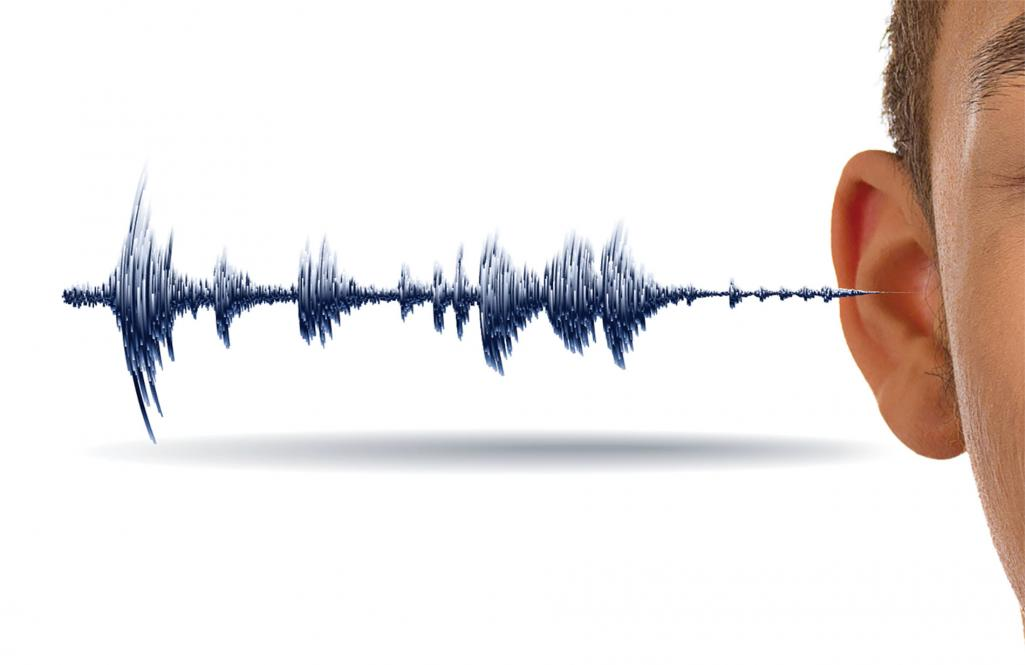
\includegraphics[width=\textwidth]{../figures/illustrations/percieving_sound}\\
  Photo Credit - \texttt{Shutterstock / mw2st / pathdoc}
}

\frame{\frametitle{Perceiving Signals}
  \centering
  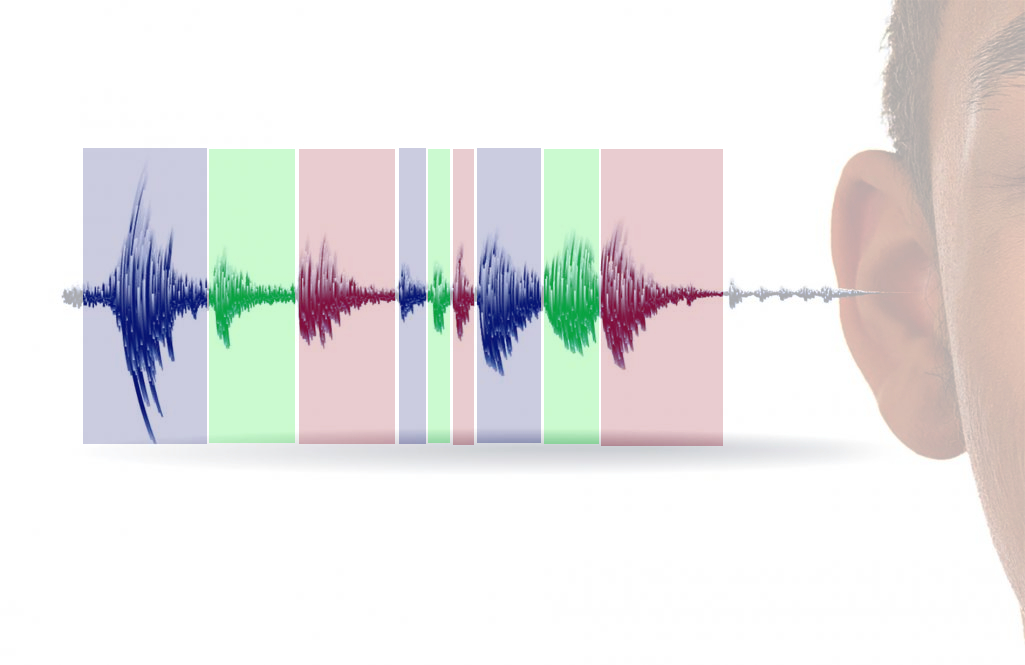
\includegraphics[width=\textwidth]{../figures/illustrations/percieving_sound2}\\
  Photo Credit - \texttt{Shutterstock / mw2st / pathdoc}
}


\section{Introduction}
\frame{\frametitle{Phrasings (Sheet Music Style).}
  \centering
  \includegraphics[height=0.3\textheight]{../figures/ly/programming_drumpatterns1}\\
  \includegraphics[height=0.3\textheight]{../figures/ly/programming_drumpatterns2}\\
  \includegraphics[height=0.3\textheight]{../figures/ly/programming_drumpatterns3}\\
}

\frame{\frametitle{Phrasing in Terms of Transformations}
  \centering
  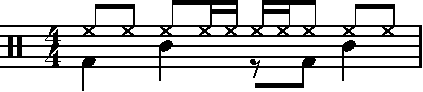
\includegraphics[width=0.8\textwidth]{../figures/ly/rock3}\\
  \vspace{0.5cm}
  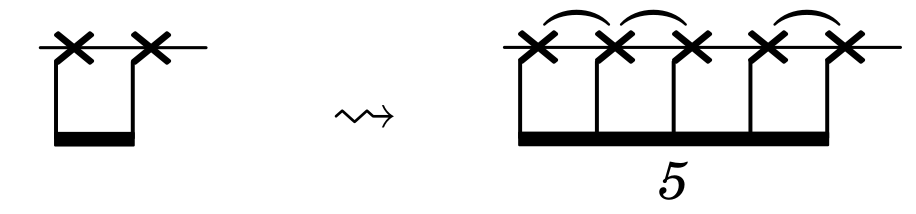
\includegraphics[width=0.6\textwidth]{../figures/illustrations/transform1337}\\
  \vspace{0.5cm}
  \includegraphics[width=0.8\textwidth]{../figures/ly/rock2_hh_shuffle}
}

\frame{\frametitle{Grid Editors}
  \centering
  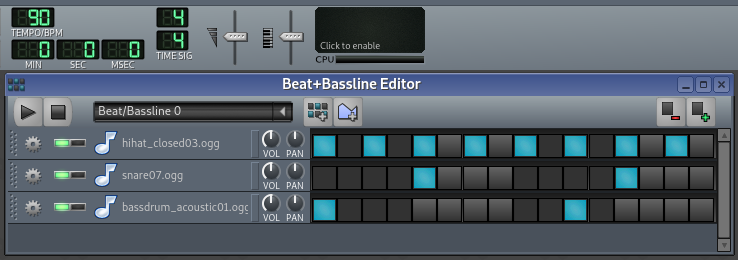
\includegraphics[width=0.8\textwidth]{../figures/illustrations/lmms/rock1}\\
  \vspace{0.5cm}
  \includegraphics[width=0.8\textwidth]{../figures/ly/rock2}
}
\frame{\frametitle{Signal Processing Languages}
  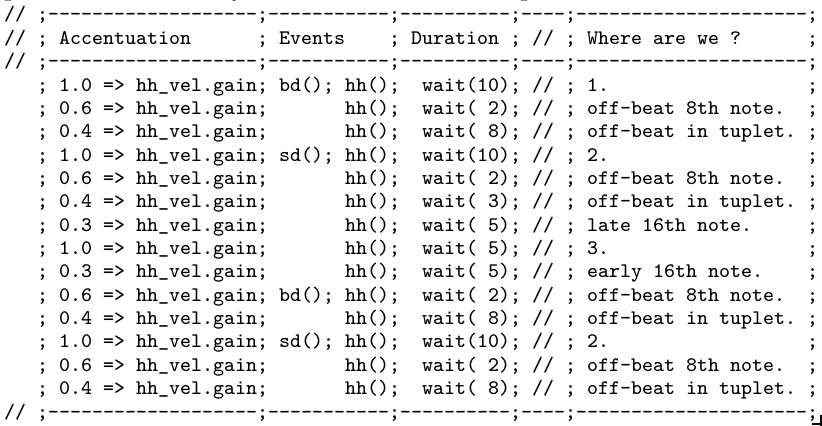
\includegraphics[width=\textwidth]{img/ChucK}
}
\frame{\frametitle{Music Score Representations and {\tt dseq}}
  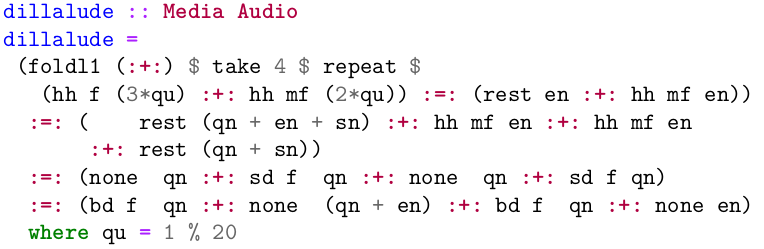
\includegraphics[width=\textwidth]{img/dillalude}\\

  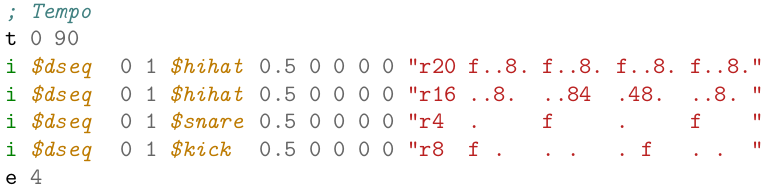
\includegraphics[width=\textwidth]{img/dseq}
}

\section{Problem Domain}
\frame{\frametitle{Analysis}
  \begin{block}{Grid Editor}
  \begin{itemize}
    \item Syntactic Overview/Constraints.
    \item Speculative Grid Selection.
    \item Specialised for Contemporary Western Music.
  \end{itemize}
  \end{block}\pause

  \begin{block}{Signal Processors}
    \begin{itemize}
      \item Full Control over Signals.
      \item Poor Structuring Mechanisms.
      \end{itemize}
  \end{block}\pause
  \begin{block}{Music Sheet Representations}
    \begin{itemize}
      \item Concise familiar notation.
      \item Trades off Syntactic Constraints for Expressive Power.
      \item Inherits Unfortunate Flaws from Sheet Music.
    \end{itemize}
  \end{block}
}

\frame{
  \frametitle{Design}
  \begin{block}{Goals:}
    \begin{itemize}
    \item Declarative.
    \item Expressive.
    \item Composable.
    \item Separation of Concerns.
    \item Preserve Alignment Constraints.
    \end{itemize}
  \end{block}
}

\frame{
  \frametitle{Lambda Cube ($\lambda_\rightarrow$)}
  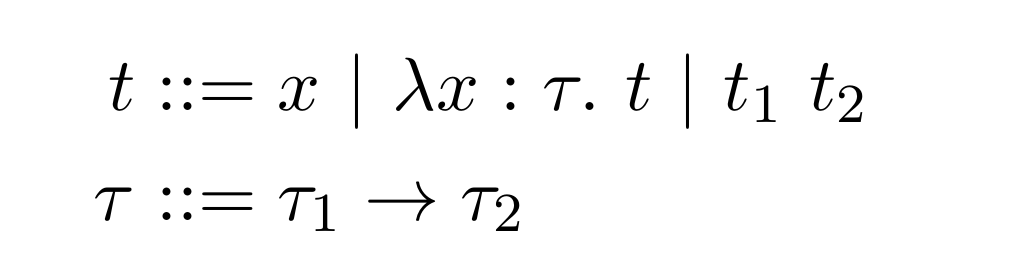
\includegraphics[width=0.5\textwidth]{../figures/illustrations/lambda_calculus/basic_syntax}\\ \\

  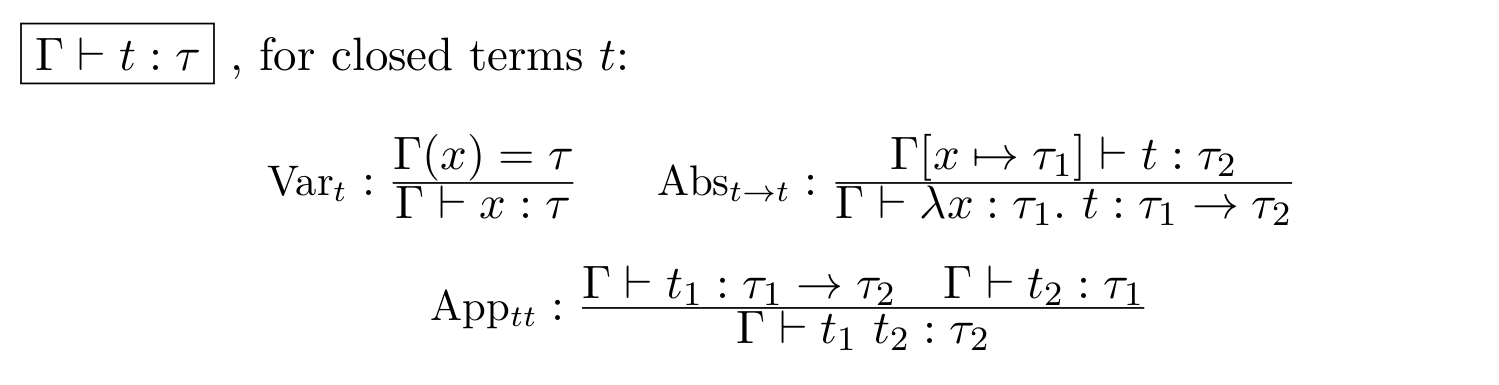
\includegraphics[width=\textwidth]{../figures/illustrations/lambda_calculus/basic_typing}
}

\frame{
  \frametitle{Lambda Cube ($\lambda_2$)}
  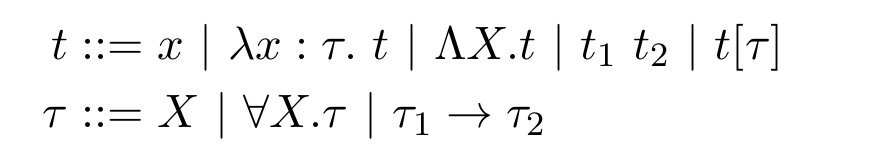
\includegraphics[width=0.5\textwidth]{../figures/illustrations/lambda_calculus/polymorphic_syntax}\\
  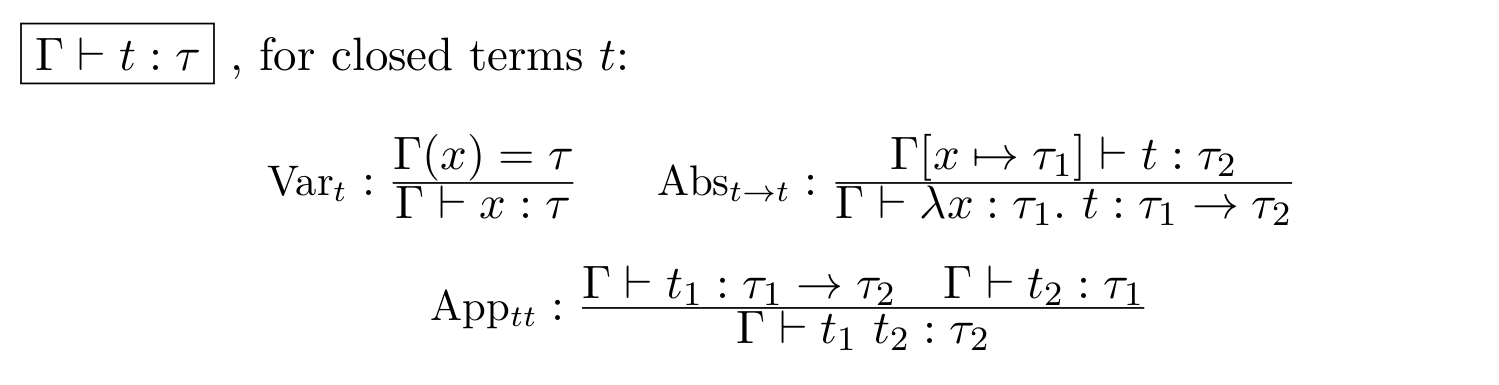
\includegraphics[width=\textwidth]{../figures/illustrations/lambda_calculus/basic_typing}\\
  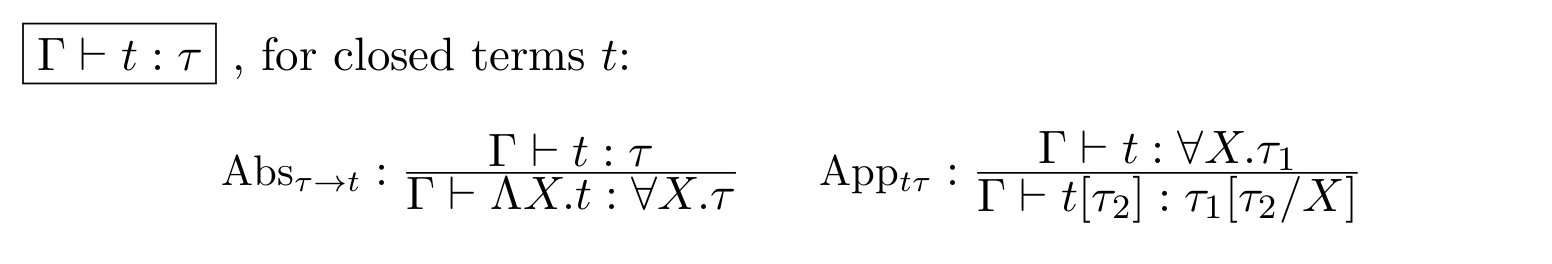
\includegraphics[width=\textwidth]{../figures/illustrations/lambda_calculus/polymorphic_typing}
}

\frame{
  \frametitle{Lambda Cube ($\lambda_\omega$)}
  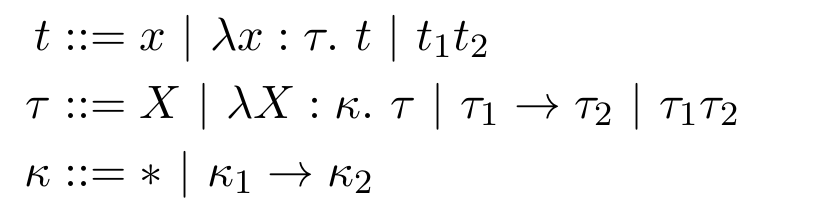
\includegraphics[width=0.5\textwidth]{../figures/illustrations/lambda_calculus/type_level_syntax}\\
  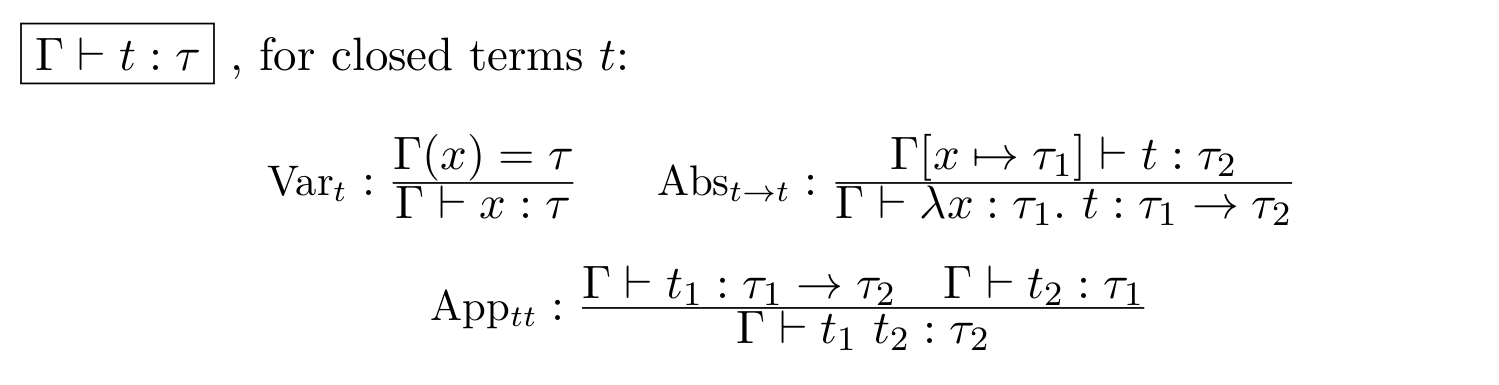
\includegraphics[width=\textwidth]{../figures/illustrations/lambda_calculus/basic_typing}\\

  repeat Var$_t$, Abs$_{t\rightarrow{t}}$ and App$_{tt}$ to get Var$_\tau$, Abs$_{\tau\rightarrow\tau}$ and App$_{\tau\tau}$.
}

\frame{
  \frametitle{Lambda Cube ($\lambda_\Pi$)}
  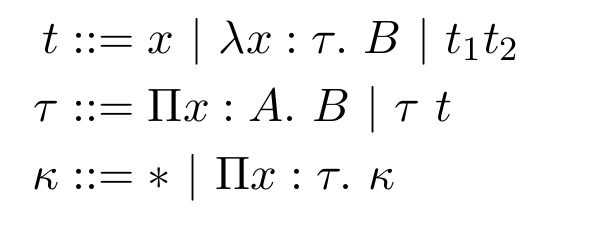
\includegraphics[width=0.5\textwidth]{../figures/illustrations/lambda_calculus/dependent_syntax}\\
  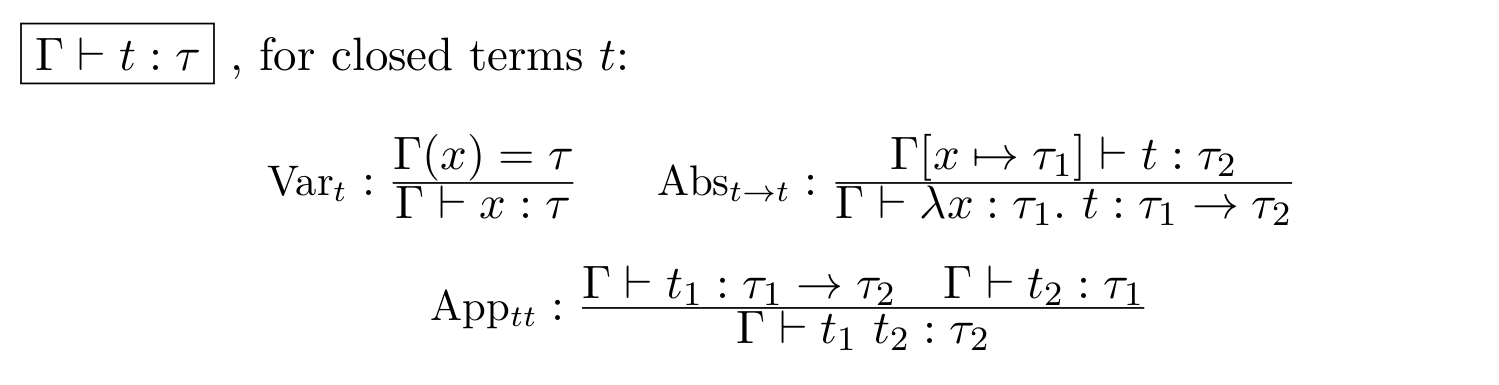
\includegraphics[width=0.9\textwidth]{../figures/illustrations/lambda_calculus/basic_typing}\\
  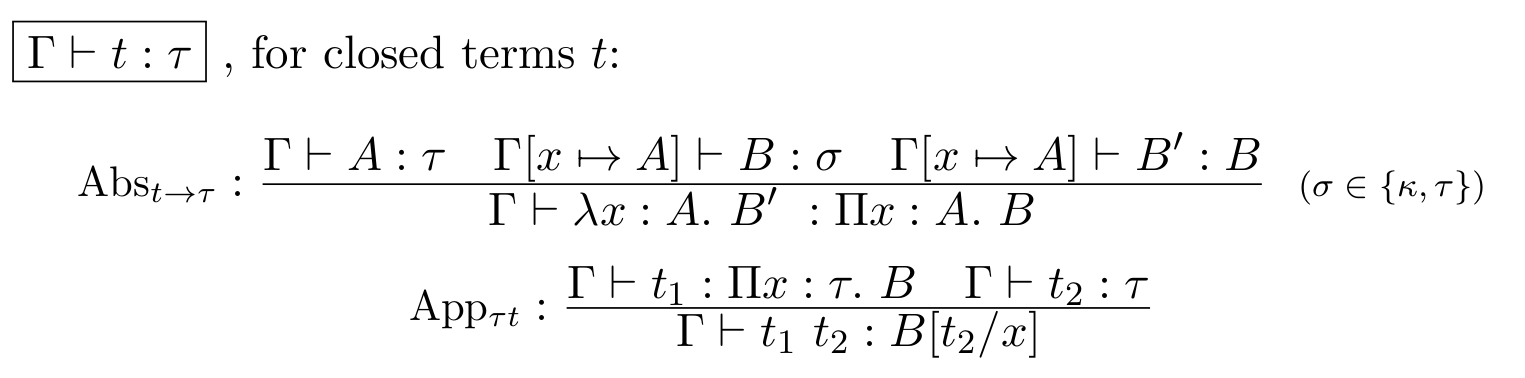
\includegraphics[width=0.9\textwidth]{../figures/illustrations/lambda_calculus/dependent_typing}
}

\begin{frame}
  \frametitle{Language overview}

  \begin{block}{Primitives:}
    \begin{itemize}
    \item Signals
    \end{itemize}
  \end{block}


  \begin{block}{User definable}
    \begin{itemize}
    \item Patterns
    \item Rhythms
    \item Grooves
    \end{itemize}
  \end{block}

\end{frame}

\frame{\frametitle{Informal Introduction}
  \centering
  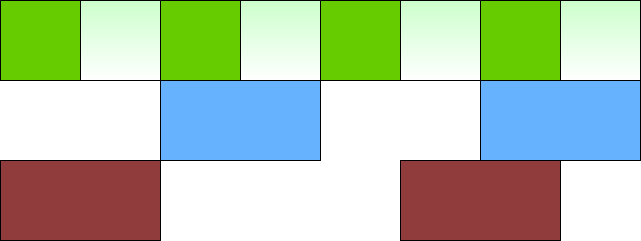
\includegraphics[width=0.8\textwidth]{../figures/illustrations/grooves/Rock1}\\
  \vspace{0.5cm}
  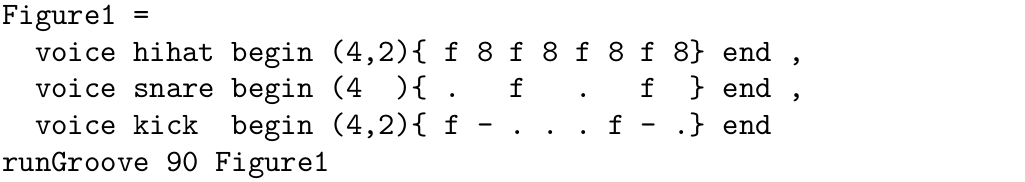
\includegraphics[width=0.8\textwidth]{../figures/illustrations/informal1_1}
}

\frame{\frametitle{Informal Introduction}
  \centering
  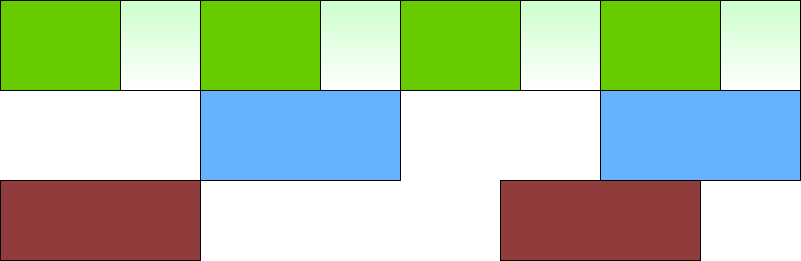
\includegraphics[width=0.8\textwidth]{../figures/illustrations/grooves/Shuffle}\\
  \vspace{0.5cm}
  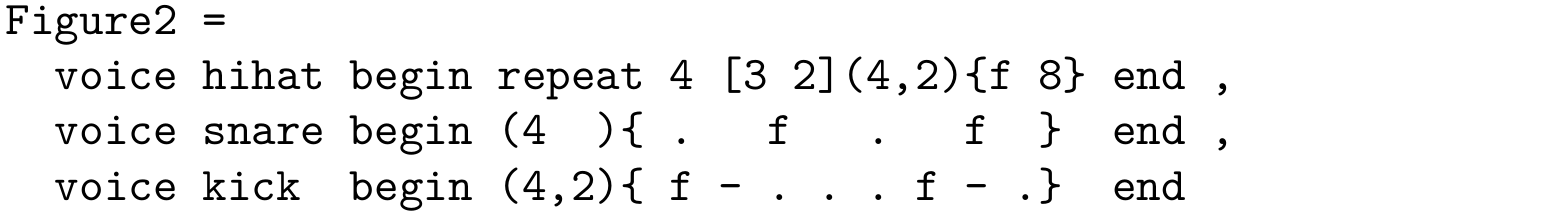
\includegraphics[width=0.8\textwidth]{../figures/illustrations/informal2_1}
}

\frame{\frametitle{Informal Introduction}
  \centering
  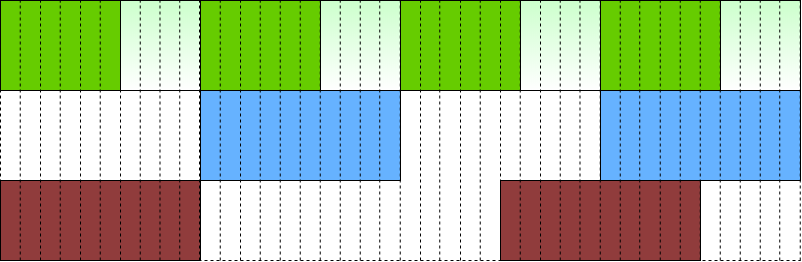
\includegraphics[width=0.8\textwidth]{../figures/illustrations/grooves/ShuffleGrid}\\
  \vspace{0.5cm}
  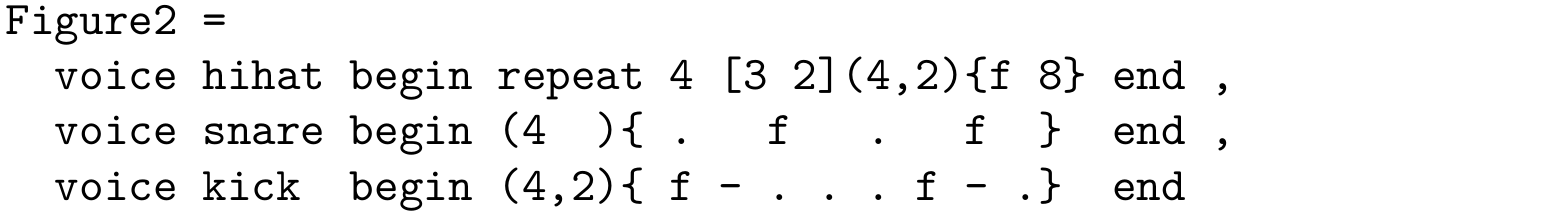
\includegraphics[width=0.8\textwidth]{../figures/illustrations/informal2_1}
}

\frame{\frametitle{Informal Introduction}
  \centering
  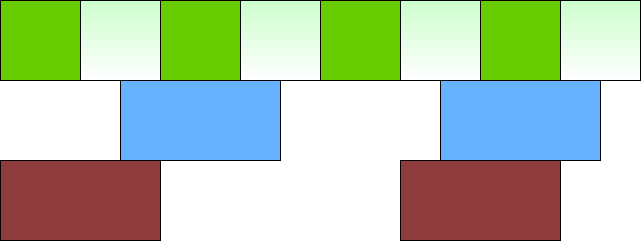
\includegraphics[width=0.8\textwidth]{../figures/illustrations/grooves/Shift}\\
  \vspace{0.5cm}
  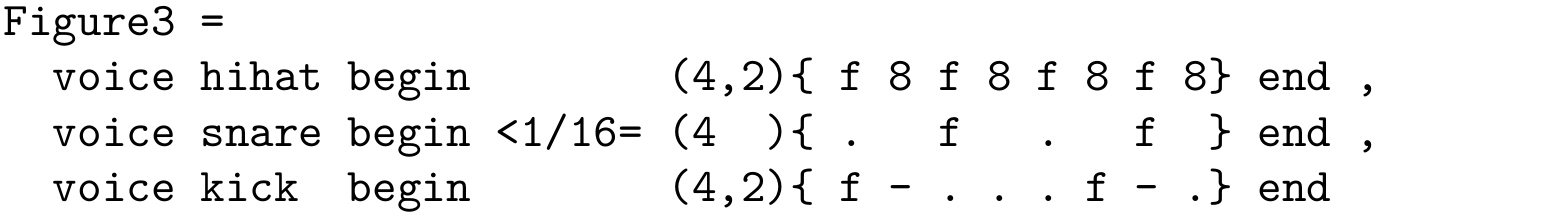
\includegraphics[width=0.8\textwidth]{../figures/illustrations/informal3_1}
}

\frame{\frametitle{Rhythms and Pulse Beats}
  \centering
  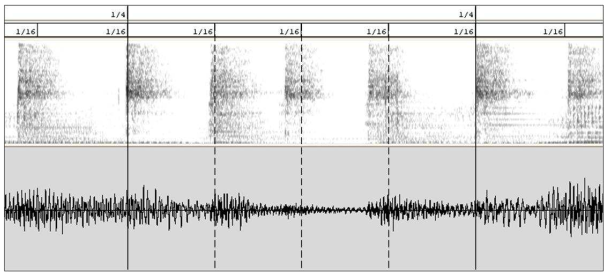
\includegraphics[width=\textwidth]{../figures/illustrations/oscilloscope/brazillian}\\
  Fabian Gouyon - Microtiming in "Samba de Roda".
}

\begin{frame}[fragile]\frametitle{$\bot$'tsh 1.0 (Syntax)}
  \begin{center}
{\scriptsize
\begin{align*}
  s &\in \Var &\text{(Well-formed signal names)}\\ a &\in \{\LIT{0}, \dots,
  \LIT{f}\} &\text{(Loudness)}\\ n,t,d &\in \N &\text{(Natural numbers)}\\ q
  &\in \mathbb Q_{\geq 0} &\text{(Fractions)}\\ ns ::&=
  \LIT{[]}\ \OR\ n\ \LIT{::}\ ns &\text{(Shapes)}\\ g ::&=
  \LIT{signature}\ n\ d
  &\text{(Grooves)}\\ &\OR\ \LIT{voice}\ s\ \LIT{begin}\ r\ \LIT{end}\\ &\OR\ \LIT{repeat}\ n\ g\\ &\OR\ g_1
  , g_2\\ &\OR\ g_1 ; g_2\\ r ::&= (n_1, n_2, \dots) \{p\}
  &\text{(Rhythms)}\\ &\OR\ [ns]\ (n_1, n_2, \dots)\{p\}\\ &\OR\ \LIT{<}
  q\LIT{=}\ r\\ &\OR\ \LIT{=}q\LIT{>}\ r\\ &\OR\ r_1\ ;
  r_2\\ p ::&=
  a\ p\ \OR\ \LIT{-}\ p\ \OR\ \LIT{.}\ p\ |\ \epsilon &\text{(Monophonic
    Metrical Patterns)}
\end{align*}
}
\end{center}
\end{frame}

\frame{\frametitle{$\bot$'tsh 1.0 (Typing)}
  \begin{align*}
    \tau := \LIT{Signal}\ |\ \LIT{Pattern}\ n\ |\ \LIT{Rhythm}\ n\ d\ |\ \LIT{Groove}\ n\ d
  \end{align*}\\
  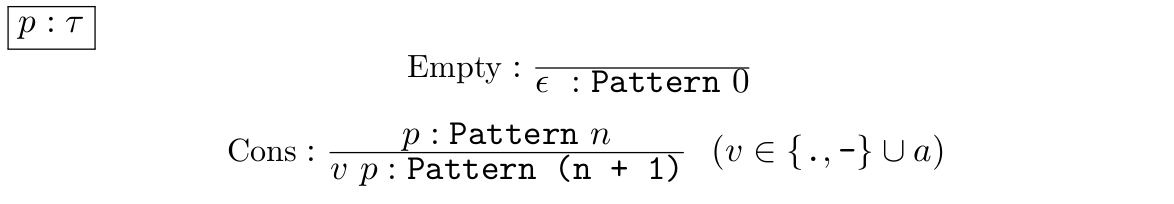
\includegraphics[width=\textwidth]{img/TypingPatterns}\\
}
\frame{\frametitle{$\bot$'tsh 1.0 (Typing)}
  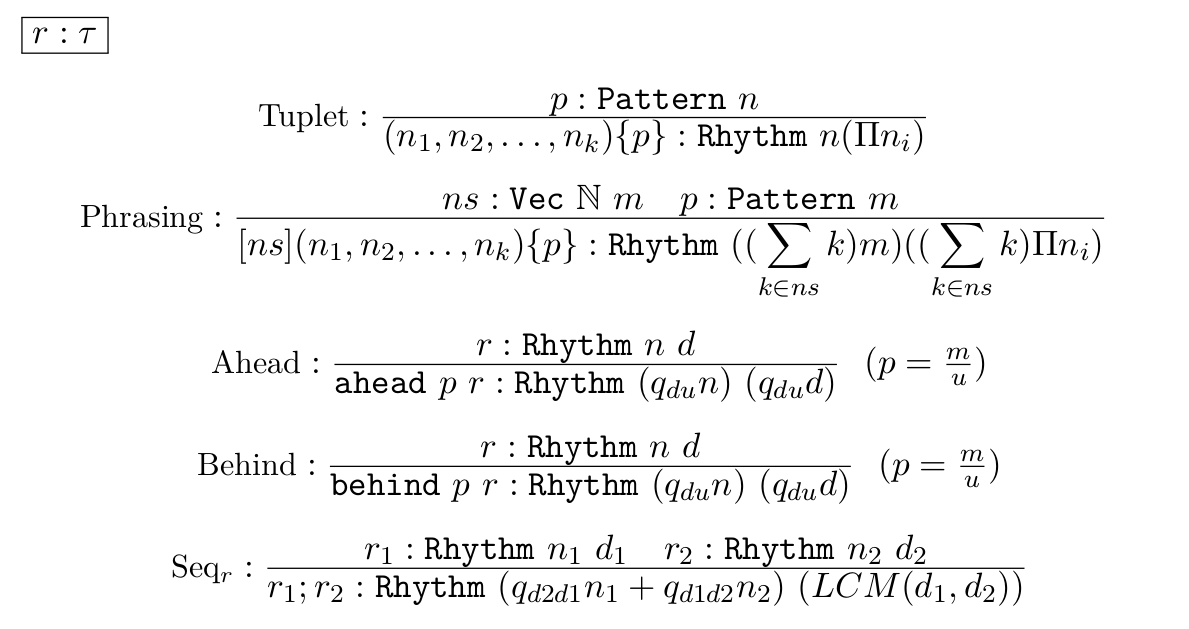
\includegraphics[width=\textwidth]{img/TypingRhythms}\\
}
\frame{\frametitle{$\bot$'tsh 1.0 (Typing)}
  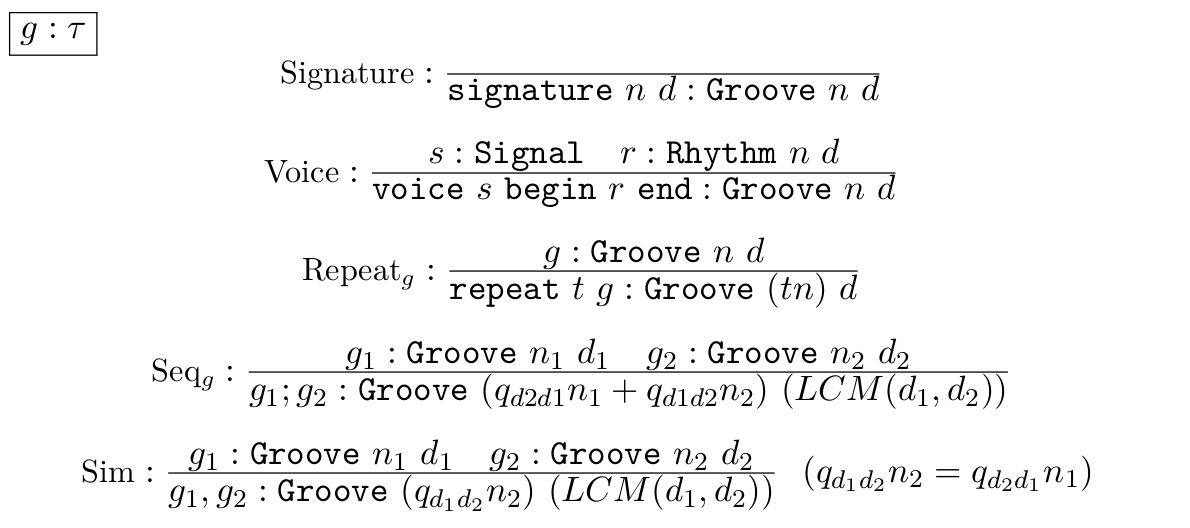
\includegraphics[width=\textwidth]{img/TypingGrooves}\\
}

\begin{frame}
  \Huge\centering
  \intro{Demonstration}
\end{frame}

\begin{frame}
  \Huge\centering
  \intro{Thank You}
\end{frame}

\begin{frame}
  \frametitle{Future}
  \begin{itemize}
    \item Euclidean Rhythms.
    \item Cabbage/VST.
    \item Metric Structures.
  \end{itemize}
\end{frame}

\end{document}

%%% Local Variables:
%%% mode: latex
%%% TeX-master: t
%%% End:
